\section{Architectural Views}
This chapter aims to provide information on the general functionalities of the proposed idea 
as well as insights on the implementation methodologies and architectural designs that will be chosen. 
To achieve this representation of the idea, the main resource used will be several UML diagrams.

Firstly, the functionalities of the system will be defined through the scenario views, thereby the logical 
view which will serve as the implementation base of the system will be designed. 
With the two views, several other views such as the process views for some use cases of the system and 
deployment designs will be presented.

All this designing will be based on the Kruchten’s 4+1 views model\cite{ArchitecturalBlueprints4+1}.

\subsection{Scenarios view: Use case analysis}

Use case diagrams are used to represent all the possible scenarios that implement the functionalities specified.

For each subsystem use case analysis, a detailed description can be found with:
\begin{itemize}
    \item Actors affected by the use-case system.
    \item The preconditions identified to achieve the functionalities described.
    \item The post-conditions.
    \item The basic flow of actions.
\end{itemize}

\subsubsection*{Soil moisture use cases}
\begin{figure}[H]
    \centering
    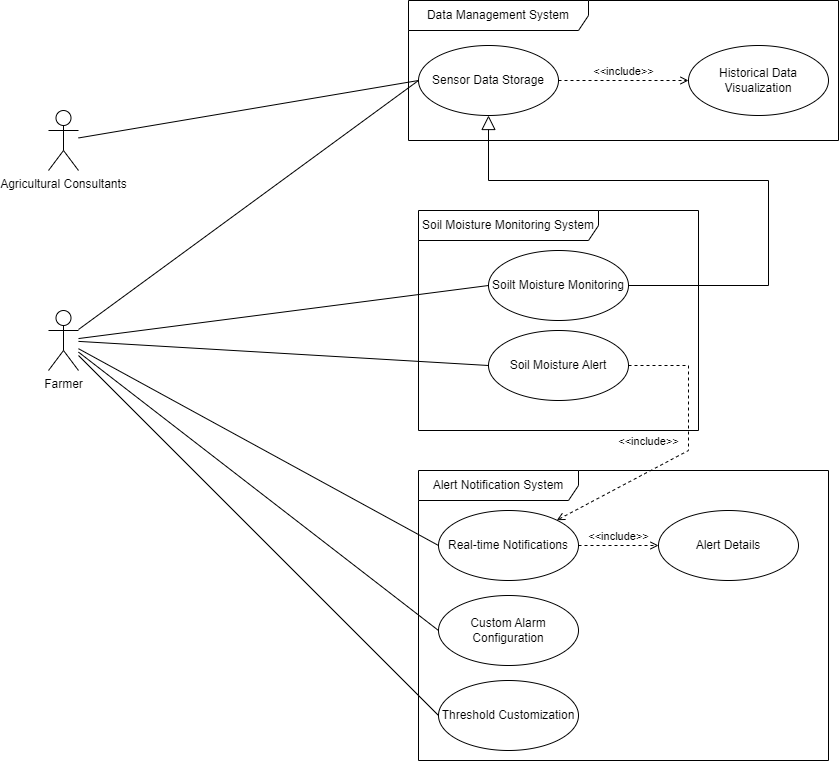
\includegraphics[width=0.7\textwidth]{./images/6/data_soil_alert_uses.png}
    \caption{Soil moisture use cases diagram}
\end{figure}
\begin{itemize}
    \item \textbf{Name}: Soil Moisture monitoring.
    \item \textbf{Actors}: Farmer.
    \item \textbf{Description}: Farmers can monitor soil moisture and review historical data. The system can generate alerts.
    \item \textbf{Pre-conditions}:
        \begin{enumerate}
            \item The soil moisture monitoring system must be operational.
            \item The system must have the alert sending function enabled.
            \item For alerts to be sent, a defined range must exist.
            \item The user must be logged into the system.
        \end{enumerate}
    \item \textbf{Basic flow of actions}:
        \begin{enumerate}
            \item The user login into the system.
            \item They can view the data.
            \item If the soil moisture values are out of range, an alert is sent.
            \item The users can view and receive the soil moisture alert.
        \end{enumerate}
\end{itemize}

\subsubsection*{Animal detection system use cases}
\begin{figure}[H]
    \centering
    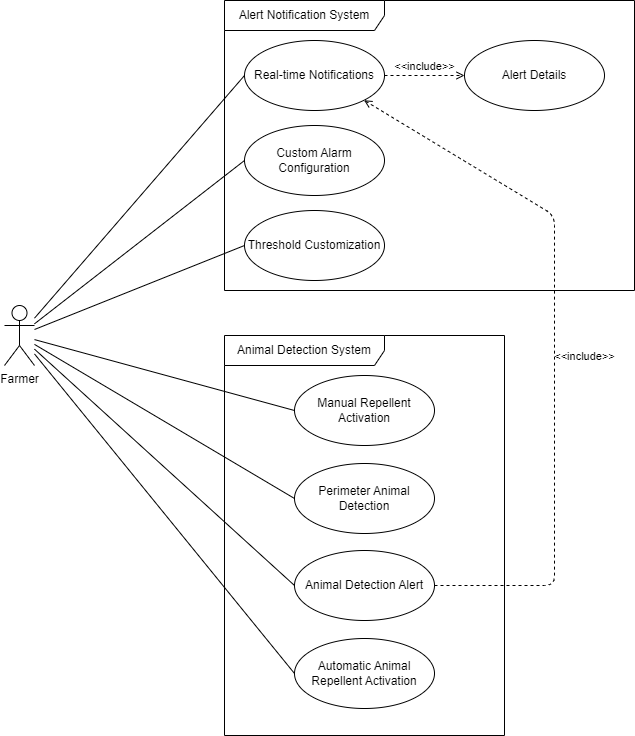
\includegraphics[width=0.8\textwidth]{./images/6/alert_animal_uses.png}
    \caption{Animal detection system use cases diagram}
\end{figure}
\begin{itemize}
    \item \textbf{Name}: Animal detection.
    \item \textbf{Actors}: Farmer.
    \item \textbf{Description}: Farmer can receive alerts of animal detection on the farm perimeter and manually or automatically configure the repulsion system.
    \item \textbf{Pre-conditions}:
        \begin{enumerate}
            \item The animal detection system must be operational.
            \item The system must have the alert sending function enabled.
            \item The user must be logged into the system.
        \end{enumerate}
    \item \textbf{Basic flow of actions}:
        \begin{enumerate}
            \item The user login into the system.
            \item The perimeter of the farm can be viewed on the map.
            \item If an animal is detected in the perimeter, an alert is sent.
            \item The user views the animal detection alert.
            \item In the map the line the perimeter changes the color in reaction to the presence.
        \end{enumerate}
\end{itemize}

\subsubsection*{User management system use cases}
\begin{figure}[H]
    \centering
    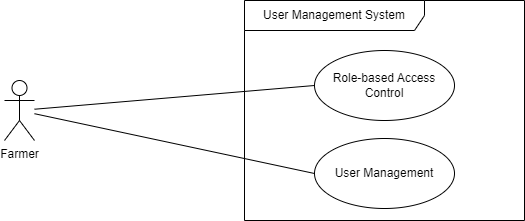
\includegraphics[width=0.95\textwidth]{./images/6/user_management_uses.png}
    \caption{User management system use cases diagram}
\end{figure}
\begin{itemize}
    \item \textbf{Name}: User Management.
    \item \textbf{Actors}: Farmer.
    \item \textbf{Description}: The farmer can configure user management and assign role access to other users.
    \item \textbf{Pre-conditions}:
        \begin{enumerate}
            \item A farmer is the administrator.
            \item The roles are defined.
            \item There must be more than one user.
            \item The user must be logged into the system.
        \end{enumerate}
    \item \textbf{Basic flow of actions}:
        \begin{enumerate}
            \item The user login into the system.
            \item The user can assign a role to another user.
        \end{enumerate}
\end{itemize}

\subsubsection*{Fire detection system use cases}
\begin{figure}[H]
    \centering
    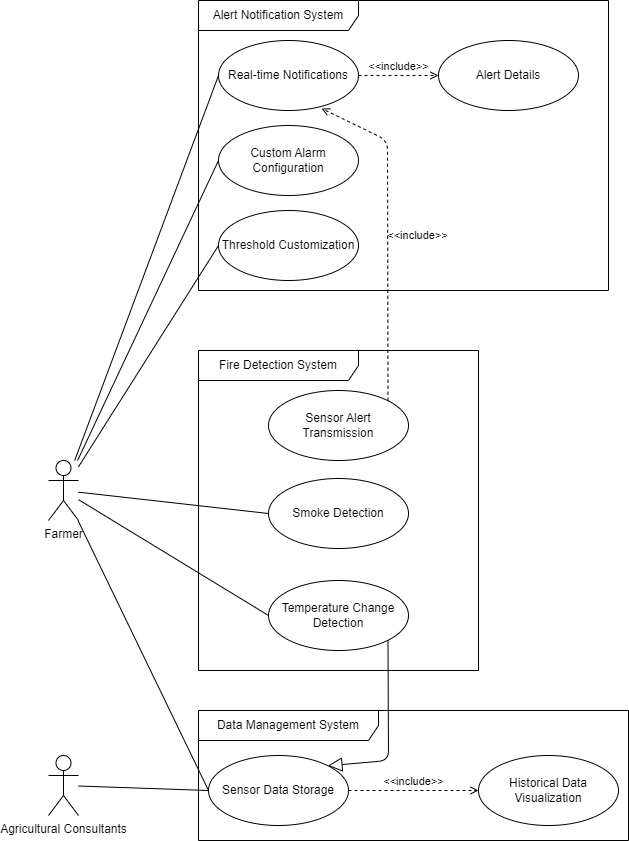
\includegraphics[width=0.98\textwidth]{./images/6/fire_uses.png}
    \caption{Fire detection system use cases diagram}
\end{figure}
\begin{itemize}
    \item \textbf{Name}: Fire Detection.
    \item \textbf{Actors}: Farmer.
    \item \textbf{Description}: The farmer can receive alerts of fire detection on the farm perimeter and can monitor the different sensors.
    \item \textbf{Pre-conditions}:
        \begin{enumerate}
            \item The fire detection system must be operational.
            \item The system must have the alert sending function enabled.
            \item The user must be logged into the system.
        \end{enumerate}
    \item \textbf{Basic flow of actions}:
        \begin{enumerate}
            \item The user login into the system.
            \item The perimeter of the farm can be viewed on the map.
            \item If a fire is detected in the perimeter, an alert is sent.
            \item The user views the fire detection alert.
            \item The fire position will be detected in the map.
        \end{enumerate}
\end{itemize}

\subsubsection*{Energy system use cases}
\begin{figure}[H]
    \centering
    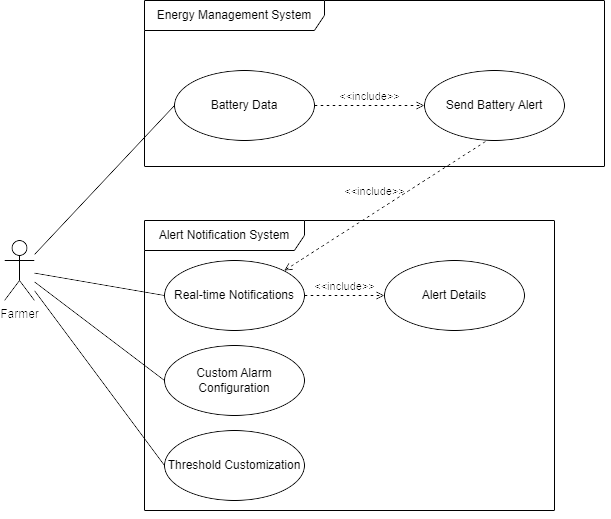
\includegraphics[width=0.78\textwidth]{./images/6/energy.png}
    \caption{Energy system use cases diagram}
\end{figure}
\begin{itemize}
    \item \textbf{Name}: Battery Management.
    \item \textbf{Actors}: Farmer.
    \item \textbf{Description}: The farmer can check the battery live and receive alerts of the battery status.
    \item \textbf{Pre-conditions}:
        \begin{enumerate}
            \item The system must have the alert sending function enabled.
            \item The user must be logged into the system.
        \end{enumerate}
    \item \textbf{Basic flow of actions}:
        \begin{enumerate}
            \item The user login into the system.
            \item The user can check the battery status of the node.
            \item If the battery is low, the system sends an alert.
        \end{enumerate}
\end{itemize}

\subsubsection*{Weather monitoring use cases}
\begin{figure}[H]
    \centering
    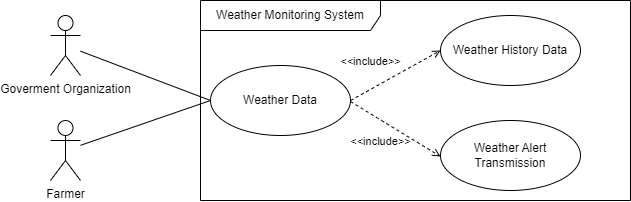
\includegraphics[width=0.95\textwidth]{./images/6/weather_uses.png}
    \caption{Weather monitoring use cases diagram}
\end{figure}
\begin{itemize}
    \item \textbf{Name}: Weather Monitoring.
    \item \textbf{Actors}: Farmer.
    \item \textbf{Description}: Farmer can monitor the weather data.
    \item \textbf{Pre-conditions}:
        \begin{enumerate}
            \item The government organization publishes weather data.
        \end{enumerate}
    \item \textbf{Basic flow of actions}:
        \begin{enumerate}
            \item The user login into the system.
            \item The user checks the weather data.
        \end{enumerate}
\end{itemize}